\quad \quad In this chapter, we will introduce a new mathematical object that you have probably heard before but not sure what it is. To be honest, many mathematics students only know how to \textit{compute} matrix operations but does not know the meaning behind them. I will try to do my best to explain them in a clear manner and I hope that you would appreciate matrices more for their beautiful geometric meaning than their mind-numbing calculations. A great place to start is the \textit{basis vectors} introduced back in \Cref{basis}. All vectors can be written as a unique linear combination of the basis vectors. But \(\ihat\) and \(\jhat\) are not the only basis vectors out there, what if I wanted to describe vectors using another set of basis vectors? Perhaps that would be more convenient for my special use case. Well, it is actually pretty easy to do so. For the sake of this argument, let us try to rotate all of the vectors in a normal 2d vector field anti-clockwise by \(90\degree\). \begin{marginfigure}
  \centering
  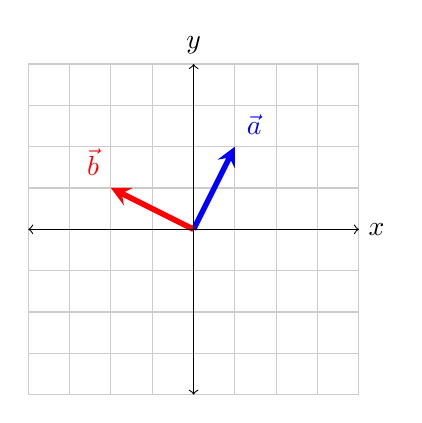
\begin{tikzpicture}[scale=0.525]
    \draw[thin, gray!40] (-4,-4) grid (4,4);
    \draw[line width=2pt, blue, -stealth] (0,0) -- (1,2) node[anchor=south west]{\(\vec{a}\)};
    \draw[line width=2pt, red, -stealth] (0,0) -- (-2,1) node[anchor=south east]{\(\vec{b}\)};
    \draw[<->] (-4,0) -- (4,0) node[right]{\(x\)};
    \draw[<->] (0,-4) -- (0,4) node[above]{\(y\)};
  \end{tikzpicture}
  \caption{Two vectors, one rotated anti-clockwise by \(90\degree\).}
  \label{rotate90}
\end{marginfigure}
Notice how we could not describe \(\vec{b}\) as some constant multiplied to \(\vec{a}\) in \Cref{rotate90}. We need some other tool to help us. If we change the basis vectors of \(\vec{a}\) to another pair of basis vectors, can we somehow get \(\vec{b}\)? Here is a thought: replace the \(\ihat\) with \(\begin{bsmallmatrix}
  0 \\
  1
\end{bsmallmatrix}\) and \(\jhat\) with \(\begin{bsmallmatrix}
  -1 \\
  0
\end{bsmallmatrix} \). So, \(\vec{a}=1\ihat+2\jhat\) will become \(\vec{a}=\begin{bsmallmatrix}
  0 \\
  1
\end{bsmallmatrix} + 2\begin{bsmallmatrix}
  -1 \\
  0
\end{bsmallmatrix} = \begin{bsmallmatrix}
  -2 \\
  1
\end{bsmallmatrix} \). This is pretty intriguing, by changing the basis vectors, we have basically "morphed" \(\vec{a}\) into \(\vec{b}\). This "morphing" is called a \textit{linear transformation} or \textit{linear map}. In some of the visualisations of the linear transformations I might keep the original grid in the background in a lighter color.


\begin{example}
  Here are some examples of linear transformations, the blue grid is the vector space after the transformation. Take note where the basis vectors are after the transformations.
  \begin{figure}[H]
  \centering
  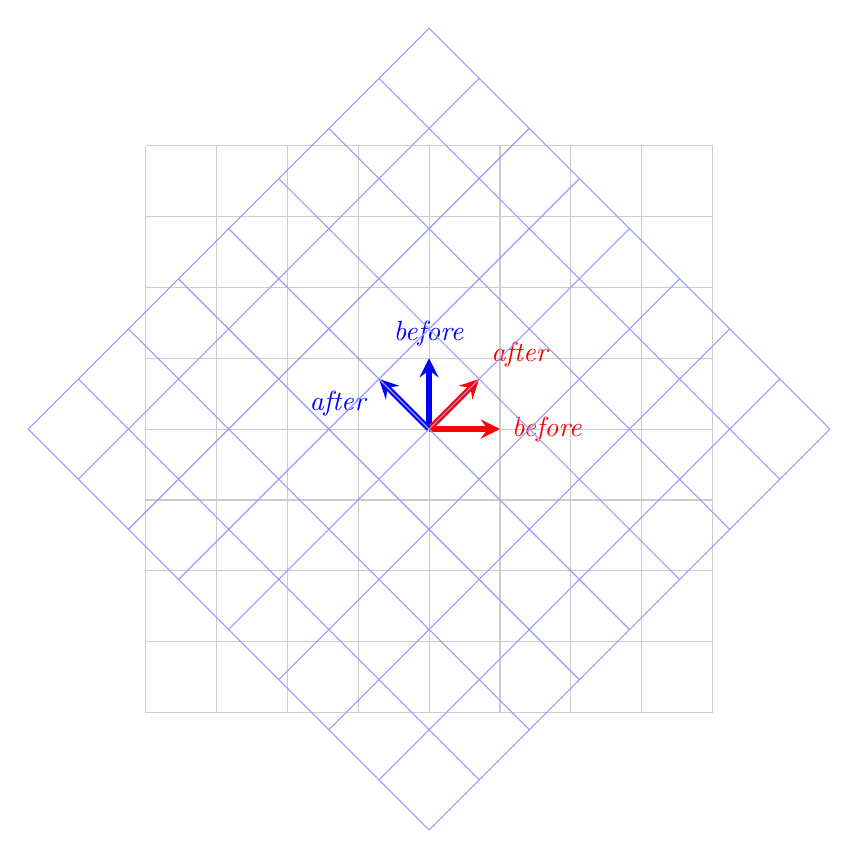
\begin{tikzpicture}[scale=0.9]
    \draw[gray!40, thin] (-4, -4) grid (4,4); 
    \draw[line width=2pt, red, -stealth] (0,0) -- (1,0) node[anchor=west]{\(\ihat_{\textit{before}}\)};
    \draw[line width=2pt, blue, -stealth] (0,0) -- (0,1) node[anchor=south]{\(\jhat_{\textit{before}}\)};
    \draw[line width=2pt, red, -stealth] (0,0) -- (0.7071068,0.7071068) node[anchor=south west]{\(\ihat_{\textit{after}}\)};
    \draw[line width=2pt, blue, -stealth] (0,0) -- (-0.7071068,0.7071068) node[anchor=north east]{\(\jhat_{\textit{after}}\)};
    \draw[blue!40, thin, rotate= 45] (-4, -4) grid (4,4);
  \end{tikzpicture}
  \caption{A transformation in the form of an anti-clockwise \textit{rotation}.}
  \end{figure}
  \begin{figure}[H]

  \centering

  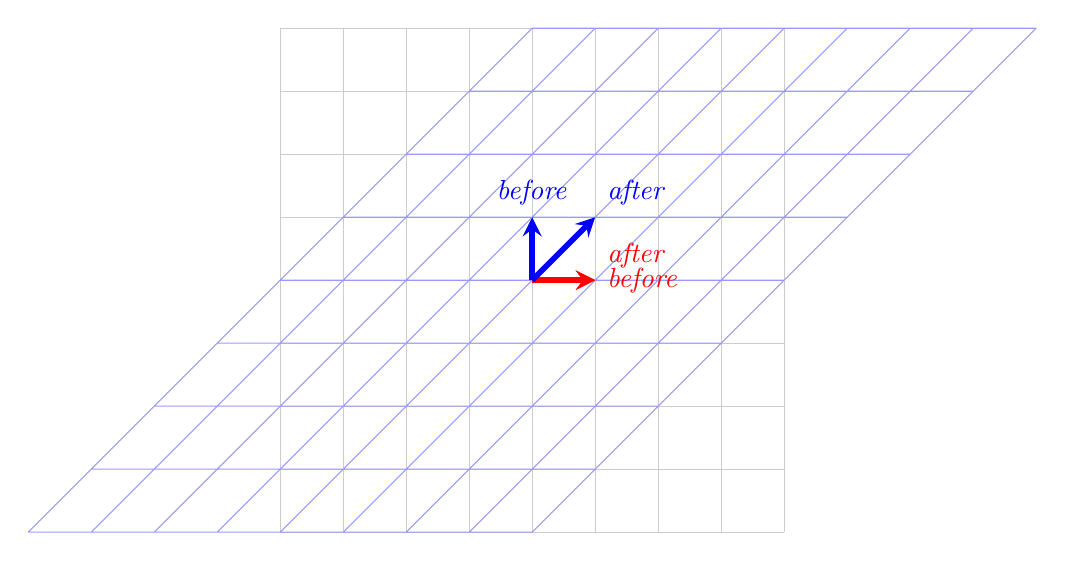
\begin{tikzpicture}[scale=0.8]
    \draw[gray!40, thin] (-4, -4) grid (4,4); 
    \draw[blue!40, thin, xslant=tan 45] (-4, -4) grid (4,4);
    \draw[line width=2pt, red, -stealth] (0,0) -- (1,0) node[anchor=west]{\(\ihat_{\textit{before}}\)};
    \draw[line width=2pt, blue, -stealth] (0,0) -- (0,1) node[anchor=south]{\(\jhat_{\textit{before}}\)};
    \draw[line width=2pt, red, -stealth] (0,0) -- (1,0) node[anchor=south west]{\(\ihat_{\textit{after}}\)};
    \draw[line width=2pt, blue, -stealth] (0,0) -- (1,1) node[anchor=south west]{\(\jhat_{\textit{after}}\)};
  \end{tikzpicture}
  \caption{A transformation in the form of a \textit{shear}.}
  \label{shearfig}

  \marginnote{\footnotesize \textit{In \Cref{shearfig}, the \(\ihat\) vector remains at the same location.}}
  \end{figure}
\end{example}


To describe these transformations, we actually only need to describe where the basis vectors land after the transformation. No other information required. We present the location of the new basis vectors in the form of a \textit{matrix}:
\begin{definition}
  In linear algebra, matrices generally represent linear transformations. A \(n \times m\) matrix is one with \(n\) rows and \(m\) columns. The nth column of the matrix denotes the representation of the corresponding basis vector after the  linear transformation.
  \begin{equation*}
    \begin{bmatrix}
      a & b \\
      c & d
    \end{bmatrix}
  \end{equation*}
  represents a matrix that moves the \(\ihat\) basis vector to \(\begin{bsmallmatrix}
    a \\
    c
  \end{bsmallmatrix} \) and moves the \(\jhat\) basis vector to \(\begin{bsmallmatrix}
    b \\
    d
  \end{bsmallmatrix} \).
\end{definition}
